\documentclass[conference]{IEEEtran}

\usepackage[utf8]{inputenc}
\usepackage[T1]{fontenc}
\usepackage{cite}
\usepackage{amsmath,amssymb}
\usepackage{graphicx}
\usepackage{textcomp}
\usepackage{booktabs}
\usepackage{array}
\usepackage{url}
\usepackage{pgfplots}
\pgfplotsset{compat=1.16}

\graphicspath{{../figs/}{figs/}}

\begin{document}

\title{A Low-Power LoRa Wireless Sensor Mesh Network with Cloud Storage for Monitoring Soil Conditions on Icelandic Turf Roofs}

\author{\IEEEauthorblockN{Jezreel V. Tan}
\IEEEauthorblockA{\textit{Faculty of Electrical and Computer Engineering} \\
\textit{School of Engineering and Natural Sciences, University of Iceland}\\
Reykjav\'ik, Iceland}}

\maketitle

\begin{abstract}
Icelandic turf houses are heritage structures whose turf roofs require maintenance and whose soil conditions are difficult to observe without disturbing the site. This paper presents the design, implementation, and evaluation of a low-cost, low-power wireless sensor network that monitors soil moisture, soil temperature, air temperature, relative humidity, and battery voltage beneath turf roofs. Sensor nodes built around an Arduino Pro Mini and a 433~MHz LoRa module exchange measurements through a ledger-based mesh protocol with CSMA/CA collision avoidance. A base station uploads the collected data to the ThingSpeak cloud platform, and each node also logs its measurements to an SD card. From the measured current in each operating state, the node's average current is calculated as 3.08~mA, giving an idealized lifetime estimate of about 142 days from three 3,500~mAh cells. Field tests observed single-hop communication at several locations within approximately 3~km, with RSSI between $-103$ and $-113$~dBm. A second-order calibration of the capacitive moisture sensor over 0--40\% gravimetric moisture has an in-sample RMSE of 3.01 percentage points. Four nodes were deployed beneath turf roofs at Keldur, and valid records spanned approximately 51 to 130 days. The results show that such a system is feasible, and they identify its main limits: calibration with site soil, packet-level logging, and multi-hop validation.
\end{abstract}

\begin{IEEEkeywords}
wireless sensor network, LoRa, mesh network, soil moisture, turf roofs, environmental monitoring, low-power systems, ThingSpeak
\end{IEEEkeywords}

\section{Introduction}
Turf construction is an important part of Icelandic architectural heritage, and the tradition is recognized on UNESCO's tentative list of World Heritage sites \cite{unesco2011turf}. Turf buildings need continued maintenance because their turf and timber elements are susceptible to moisture-related deterioration, and the water retention of turf materials is an active research topic \cite{lin2023turf}. Their architecture, building technology, and indoor environment have also been studied \cite{vanhoof2008turf}. Understanding the moisture and temperature conditions under a turf roof therefore supports conservation, but the sites are remote, often open to the public, and must not be visually or physically disturbed. Manual sampling is infrequent and intrusive, and commercial logging systems can be costly for small research teams.

This work presents a low-cost, low-power monitoring system that is concealed beneath the turf, communicates over LoRa, and makes its measurements remotely available through a cloud platform. The system was developed in cooperation with the National Museum of Iceland and was deployed at the Keldur turf-house site. Its contribution is the integration of readily available components into a deployable platform, together with an experimental account of its power consumption, communication range, sensor calibration, cloud upload, and field behavior. It does not introduce a new sensing principle or radio technology. The paper also reports the limitations of the evidence collected, so that the results are not overstated.

The remainder of the paper is organized as follows. Section~\ref{sec:related} reviews related work. Section~\ref{sec:design} describes the system design. Section~\ref{sec:method} describes the experimental methods. Section~\ref{sec:results} presents the results, Section~\ref{sec:discussion} discusses limitations, and Section~\ref{sec:conclusion} concludes the paper.

\section{Related Work}\label{sec:related}
\subsection{LoRa and LoRa Mesh Networks}
LoRa offers long range and low power consumption for low-bandwidth applications, and its range can reach several kilometers depending on the antenna, radio configuration, terrain, and environment \cite{centenaro2016longrange}. Standard LoRaWAN uses a star-of-stars topology, whereas multi-hop and mesh extensions have been proposed to extend coverage and reduce reliance on a single path \cite{centelles2021multihop,sole2022mesh,zhu2019mesh}. Mesh strategies have been reported to improve performance in air-quality monitoring \cite{mullick2022mesh}, to roughly double the range of an asset-tracking prototype \cite{andersen2020mesh}, and to support long-distance multi-hop wildfire sensing \cite{khonrang2022multihop}. Multi-hop operation also adds latency, because nodes must coordinate transmissions and avoid collisions \cite{centelles2021multihop}. Low-cost, low-power LoRa systems have also been used for groundwater monitoring \cite{kombo2021groundwater}.

\subsection{Low-Cost Capacitive Soil Moisture Sensing}
Capacitive sensors respond to the dielectric permittivity of the soil, which increases with water content \cite{gonzalezteruel2019sdi12}. Low-cost capacitive sensors have been proposed for smart agriculture, but they require calibration to give meaningful values \cite{kulmany2022capacitive}. Calibration against the gravimetric method and professional-class reference instruments is therefore a necessary part of using such sensors.

\subsection{Positioning of This Work}
The reviewed technologies are individually established. This paper combines them in a mesh-based, SD-backed, cloud-connected node concealed beneath turf roofs, and it reports measured and observed behavior from laboratory tests and a field deployment on a heritage site.

\section{System Design}\label{sec:design}
\subsection{Requirements and Architecture}
The monitoring system must (i) measure soil moisture, soil temperature, air temperature, and relative humidity; (ii) deliver data reliably despite disturbances between nodes; (iii) operate for extended periods with sparse maintenance; (iv) retain data locally when transmissions are missed; and (v) make data available to researchers remotely. The nodes must be concealed beneath the turf, withstand moisture, freezing and thawing, and snow, and be installed non-destructively.

Fig.~\ref{fig:concept} shows the architecture. Sensor nodes form a LoRa mesh and pass data between neighbors until it reaches the base station, which uploads it to a cloud database that users access through a website.

\begin{figure}[t]
\centering
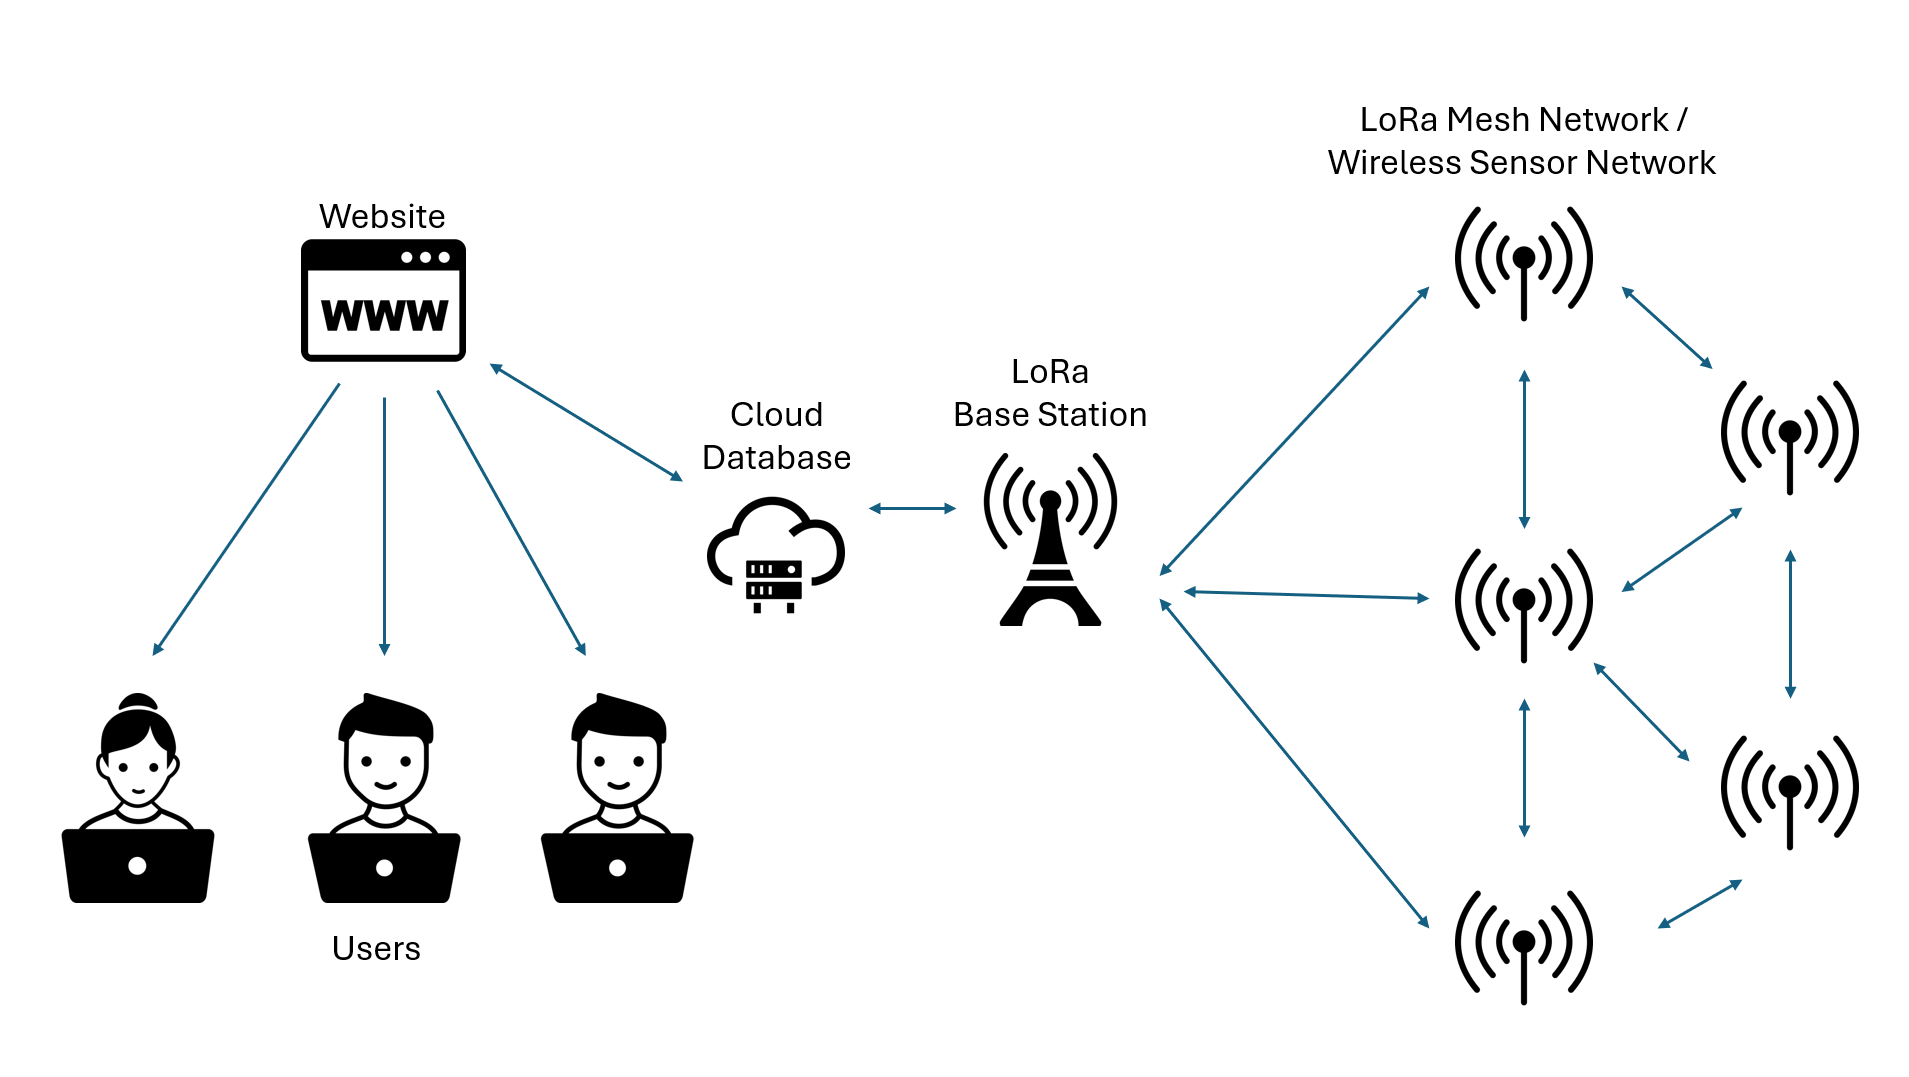
\includegraphics[width=\columnwidth]{method-image1.png}
\caption{System concept: a LoRa mesh of in situ sensor nodes, a base station, and a cloud database accessed by users.}
\label{fig:concept}
\end{figure}

\subsection{Sensor Node Hardware}
A node (Fig.~\ref{fig:node}) is built around an Arduino Pro Mini (ATmega328P, 3.3~V, 8~MHz). An ESP32 was considered but rejected because of higher power consumption and cost. Table~\ref{tab:components} lists the components. All components operate at 3.3~V or below. Two MOSFET-switched power groups (sensors and LoRa module) are disabled during sleep, and the DS3231 real-time clock wakes the microcontroller through its alarm interrupt. A custom PCB integrates the components, and a three-bit switch sets the hardware ID, so up to eight sensor nodes (IDs 0--7) are supported.

\begin{figure}[t]
\centering
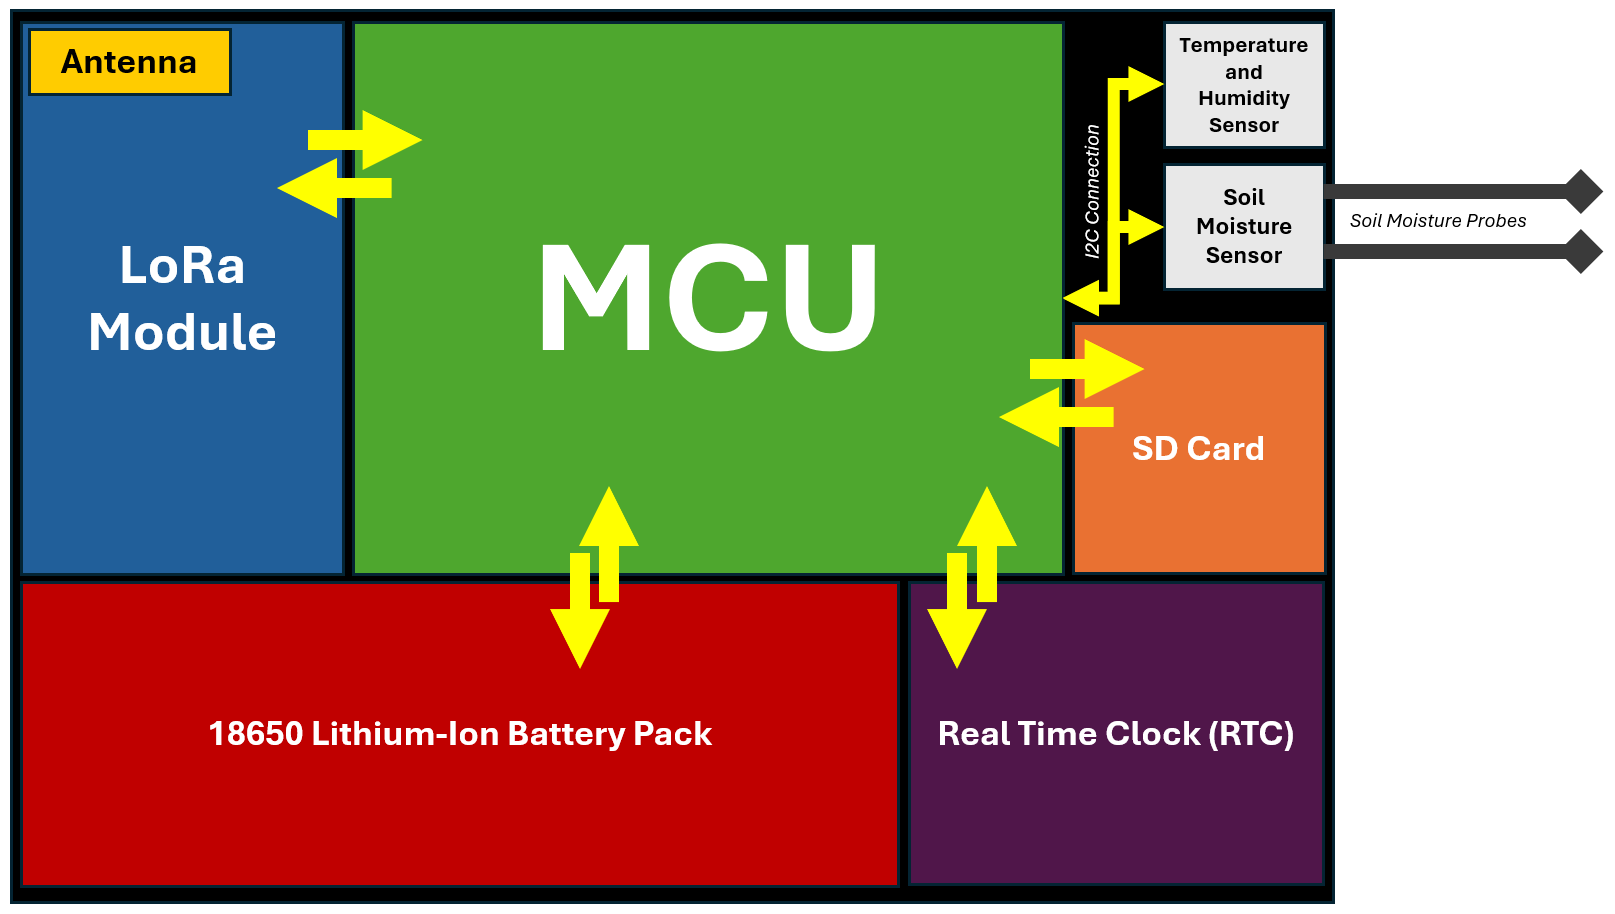
\includegraphics[width=0.9\columnwidth]{method-image2.png}
\caption{In situ sensor node hardware configuration.}
\label{fig:node}
\end{figure}

\begin{table}[t]
\caption{Sensor Node Components}
\label{tab:components}
\centering
\small
\begin{tabular}{@{}p{0.34\columnwidth}p{0.58\columnwidth}@{}}
\toprule
Function & Component \\
\midrule
Microcontroller & Arduino Pro Mini (ATmega328P) \\
Radio & Ra-02 (SX1278), 433~MHz, 3~dBi antenna \\
Soil moisture & Capacitive sensor v1.2 (analog) \\
Soil temperature & DS18B20 (1-Wire, $\pm$0.5~\textdegree C) \\
Air temp./humidity & AHT10 (I$^2$C, $\pm$0.3~\textdegree C, $\pm$2\%) \\
Local storage & SparkFun OpenLog microSD logger \\
Timekeeping & DS3231 real-time clock \\
Power & Three 18650 cells in parallel, 10,500~mAh \\
\bottomrule
\end{tabular}
\end{table}

Soil moisture is read through the 10-bit ADC. Battery voltage is measured through a 10~k$\Omega$/33~k$\Omega$ divider. Capacitive sensors were chosen over resistive ones for their lower susceptibility to corrosion, and over TDR and FDR instruments for cost and scalability.

The base station uses a LOLIN D1 mini (ESP8266) with the same Ra-02 module. It obtains the time from an NTP server, initiates each data-collection cycle, and uploads the result to ThingSpeak \cite{thingspeak} over Wi-Fi using HTTP GET requests, one request per active node. The firmware was developed in C/C++ with the Arduino IDE and uses the Arduino LoRa library \cite{mistry_arduinolora}; it is publicly available \cite{turfroof_lora}.

\subsection{Duty Cycle and Time Synchronization}
Each node is active for at most 5 minutes per hour and otherwise in deep sleep. After the base station completes a collection cycle, it distributes the NTP time in a date packet, which nodes use to update their RTCs and which can propagate through the mesh. This keeps the nodes aligned so that they wake together.

\subsection{Ledger-Based Mesh Protocol}
The mesh protocol is inspired by distributed ledgers, but it does not implement blockchain or consensus. The base station initiates a collection cycle by broadcasting a ledger template with one fixed field per hardware ID plus a checksum field. Each node keeps a local copy. On receiving a valid ledger, a node merges any entries it does not yet hold, fills the ledger with entries it already knows, recalculates the checksum, and relays the ledger only if it differed from its local database. An identical ledger is ignored, which prevents rebroadcast loops. If a node receives a ledger that lacks data it already holds, it can supply that data directly instead of waiting for it to travel back from the source. In a linear topology, the ledger propagates outward and the completed ledger propagates back to the base station. A node's measurements may therefore reach the base station directly or through intermediate nodes, and a lost packet can be recovered from neighboring nodes in later transmissions.

\textit{Packet format.} Packets are 96-byte human-readable text fields in brackets, with a header that identifies the data type. Values use fixed-width fields covering $-99.9999$ to $999.9999$. The checksum is the arithmetic sum of the node fields from 0 through 7, chosen over CRC16 to limit computation on the ATmega328P. A text format is less efficient than a packed binary payload, but it simplified debugging of routing and formatting. Before transmission, packets are encrypted with an RC4 routine, which provides basic obfuscation only; RC4 was used because AES exceeded the RAM and CPU resources of the microcontroller.

\textit{Collision avoidance.} Because the radio cannot transmit and receive simultaneously, nodes use CSMA/CA. A node senses the channel and, if it is busy, waits for a timeout equal to a base value multiplied by its hardware ID, so that timeouts differ between nodes. A node that receives a valid packet while waiting re-evaluates it and restarts its timeout. Rare simultaneous transmissions remain possible, but they are recoverable through relaying.

\subsection{Radio Configuration}
All range tests used 433~MHz, 17~dBm transmit power, 125~kHz bandwidth, spreading factor 10, coding rate 4/5, an 8-symbol preamble, and sync word 0x12. The 433~MHz band is permitted for this use in Iceland.

\section{Experimental Methods}\label{sec:method}
\subsection{Power Consumption}
The current of each operating state was measured in the laboratory, holding each state for 10~s to let the reading stabilize and observing three complete loops for repeatability. The average current is a weighted average over the hourly operating cycle, not a continuous one-hour measurement. The time-on-air of one 96-byte packet was calculated with the Semtech equations for the SX1276/77/78/79 family \cite{semtech2020sx1276}.

\subsection{Field Tests}
Preliminary and intermediate tests on the University of Iceland campus used four prototype nodes 50--100~m from the base station to validate hardware and firmware, and nearby Icelandic Meteorological Office stations served as contextual references \cite{imo_observations}. A LoRa range test was then carried out in a semi-urban area around Vellir in Hafnarfj\"{o}r\dh ur, recording RSSI at several locations. Mesh forwarding was not enabled during that test, so it evaluated single-hop communication only.

The long-term deployment began on 17 October 2025 at Keldur. Four nodes (IDs 1, 3, 5, 7) were installed beneath four turf roofs, with soil sensors at depths from approximately 60 to 85~mm. Nodes 1 and 3 had the air temperature and humidity sensor inside the waterproof enclosure; on nodes 5 and 7 it was mounted externally. Weather data were taken from the S\'amssta\dh ir station (6222) \cite{imo_observations}, which is 9.75~km from the site and was therefore a contextual reference rather than a calibration source.

\subsection{Soil Moisture Calibration}
Gravimetric calibration used a separate Icelandic soil sample at 0, 10, 20, 30, and 40\% moisture. Calibration stopped at 40\% because the soil approached saturation and additional water produced little dielectric change. Test 1 used a 2069.5~g sample with two capacitive sensors, and Test 2 used a 400~g sample with one sensor. A HOBO MX2307 logger \cite{onset_mx2307} served as a reference trend; its reported volumetric water content was converted to estimated permittivity with the Topp relationship \cite{topp1980}. A second-order polynomial was fitted to the mean ADC readings of Test 1.

\section{Results}\label{sec:results}
\subsection{Power Consumption and Estimated Lifetime}
With $SF=10$ and $BW=125$~kHz, the symbol time is $T_{sym}=2^{SF}/BW=8.192$~ms. The 96-byte packet takes 108 payload symbols, giving a time-on-air of approximately 0.985~s. The hourly budget instead allocates a conservative 60~s to the radio-active state, covering reception, transmission, relaying, processing, and overhead. Table~\ref{tab:modes} lists the measured currents and durations.

\begin{table}[t]
\caption{Operating States and Hourly Cycle}
\label{tab:modes}
\centering
\small
\begin{tabular}{@{}p{0.43\columnwidth}cc@{}}
\toprule
State & Current (mA) & Time per hour \\
\midrule
Deep sleep (all modules off) & 0.3 & 55 min \\
Awake (sensors on, LoRa off) & 9.5 & 3 s \\
LoRa RX/TX (allocation) & 119.5 & 60 s \\
Half sleep (radio in receive) & 12.2 & 237 s \\
\bottomrule
\end{tabular}
\end{table}

The weighted average current is
\begin{equation}
I_{avg}=\frac{\sum_n I_n t_n}{3600\,\mathrm{s}}\approx 3.08\ \mathrm{mA}.
\end{equation}
For three 3,500~mAh cells in parallel (10,500~mAh), the idealized lifetime is $10{,}500/3.08\approx 3409$~h, or about 142 days. A single cell would give about 47 days. This estimate assumes ideal battery behavior and excludes the capacity loss expected at low temperatures, and it is not a measured lifetime of the final three-cell configuration. In preliminary tests, single-cell nodes logged operating periods of 11 to 27 days on the SD card (the longest was 26.8 days, with the voltage falling from 4.136~V to 3.560~V). These are observed operating periods during development, not full-discharge lifetimes.

\subsection{LoRa Range}
Successful single-hop communication was observed at several test locations within approximately 3~km. Average RSSI values were $-103$~dBm at Holt and Vatnsl\'i\dh, $-112$~dBm at the fish drying area and Netto, and $-113$~dBm at \'Asvallalaug. Signal quality improved with elevated node placement, and occasional packet loss occurred where buildings or terrain obstructed the path (Fig.~\ref{fig:map}). Packet delivery percentages and per-location packet counts were not recorded, so the test does not show uniform reliability over the whole 3~km area. The antennas supplied initially were designed for Wi-Fi rather than 433~MHz, and replacing them with 433~MHz antennas improved communication reliability substantially.

\begin{figure}[t]
\centering
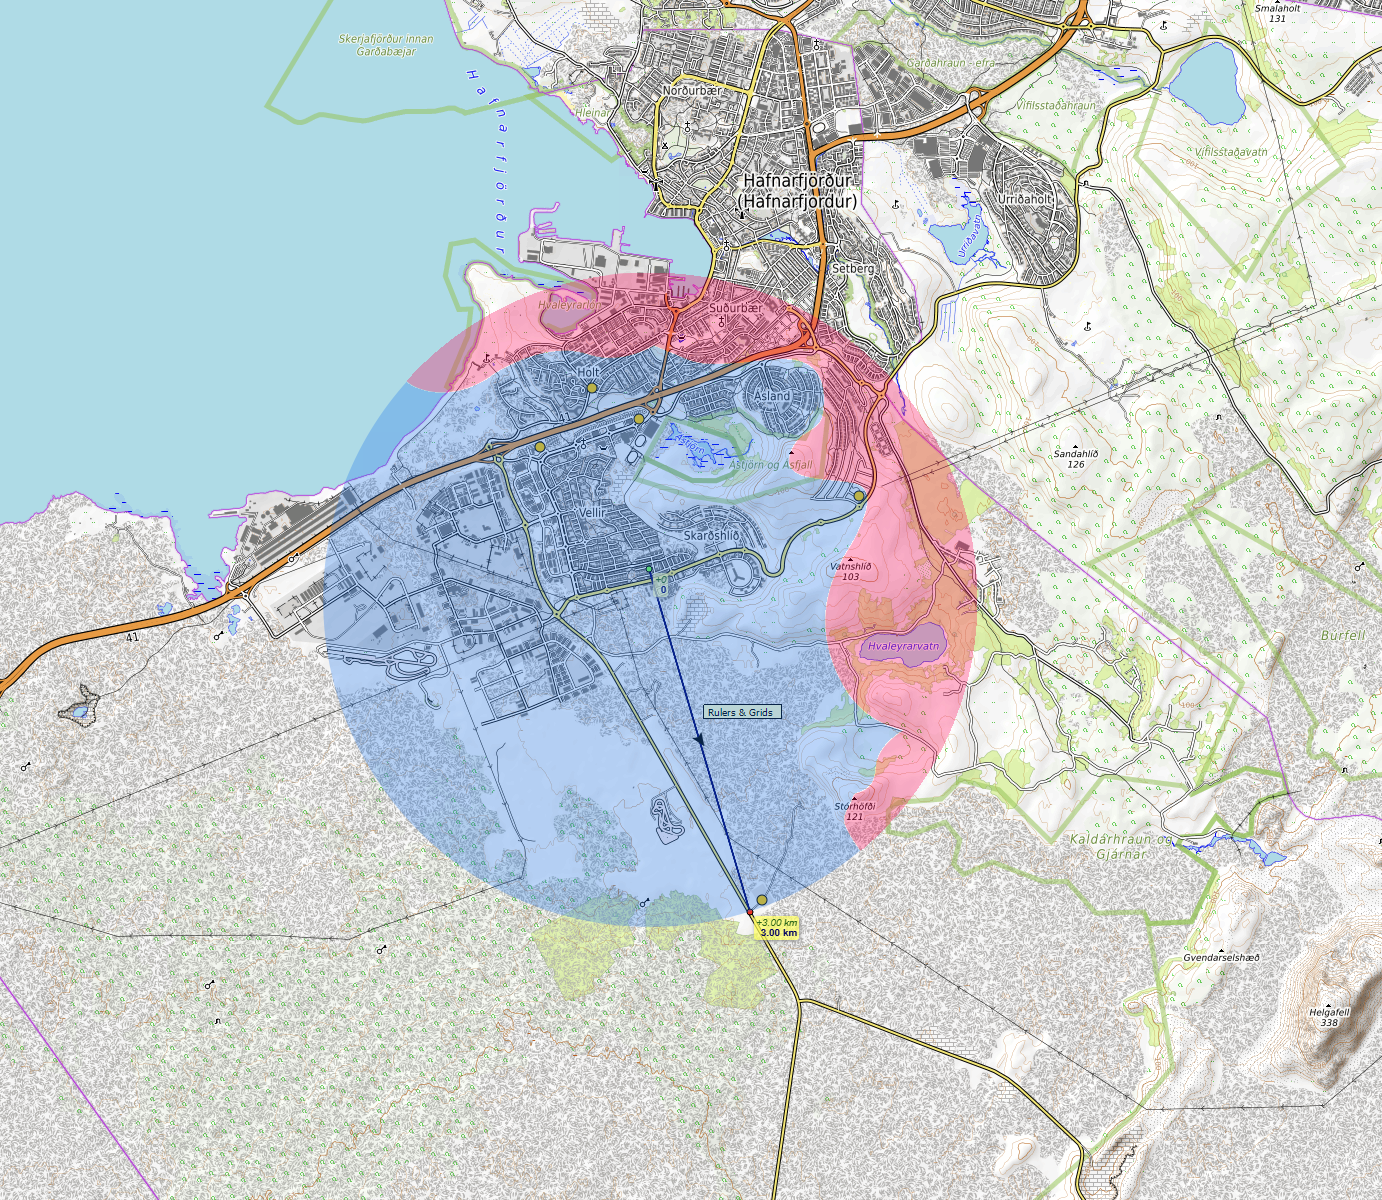
\includegraphics[width=\columnwidth]{results-image5.png}
\caption{Indicative LoRa coverage map for the Vellir test. It is based on the tested locations and is not a measured coverage boundary.}
\label{fig:map}
\end{figure}

Mesh relay was observed only qualitatively, through debug output on the bench in which ledger data were forwarded between nodes until they reached the base station. No logs were retained, so no multi-hop range, delivery ratio, hop count, or latency is reported.

\subsection{Keldur Deployment}
Table~\ref{tab:keldur} summarizes the valid ThingSpeak records of the four nodes. The elapsed spans (first to last valid record) range from approximately 50.9 to 129.5 days. They include missing records and are not uninterrupted operating times or confirmed battery lifetimes. The final battery voltages (3.49 to 3.93~V) all remained above the configured 3.25~V cutoff, and because the nodes were not retrieved, the reason that each stopped reporting is unknown. A common interruption of approximately 145 hours appeared in the records of nodes 1, 3, and 5 between 17 and 23 December 2025, but with no retained base-station logs it cannot be attributed to the LoRa link, the base station, or the internet connection.

\begin{table}[t]
\caption{Valid ThingSpeak Records at Keldur}
\label{tab:keldur}
\centering
\small
\begin{tabular}{@{}cllcc@{}}
\toprule
Node & First & Last & Span (days) & Final (V) \\
\midrule
1 & 17 Oct 2025 & 26 Dec 2025 & 70.8 & 3.63 \\
3 & 17 Oct 2025 & 23 Feb 2026 & 129.5 & 3.49 \\
5 & 17 Oct 2025 & 2 Jan 2026 & 77.5 & 3.78 \\
7 & 17 Oct 2025 & 6 Dec 2025 & 50.9 & 3.93 \\
\bottomrule
\end{tabular}
\end{table}

\textit{Air temperature and humidity.} Nodes 5 and 7, with externally mounted sensors, followed the broader variations of the S\'amssta\dh ir station and showed clearer daily fluctuation than nodes 1 and 3, whose enclosed sensors gave smoother curves. The mean absolute difference from the station ranged from 3.06 to 3.27~\textdegree C, which reflects the separation between the two locations and is not a measure of sensor accuracy. The deployment was not a controlled placement experiment, so differences in exposure may also have contributed. Node 3 reported relative humidity near 100\% for an extended period toward the end of its record, and these values should not be treated as reliable. The cause could not be determined.

\textit{Soil temperature.} All four nodes behaved similarly regardless of configuration (Fig.~\ref{fig:temps}). Soil temperature stayed close to 0~\textdegree C for much of the period while air temperature varied between about $-8$ and $+10$~\textdegree C, which is consistent with the thermal buffering of the turf and soil. The station provides only ground-surface temperature rather than temperature at the sensor depth, so the 2.77 to 3.11~\textdegree C mean absolute difference is not an accuracy measure.

\begin{figure*}[t]
\centering
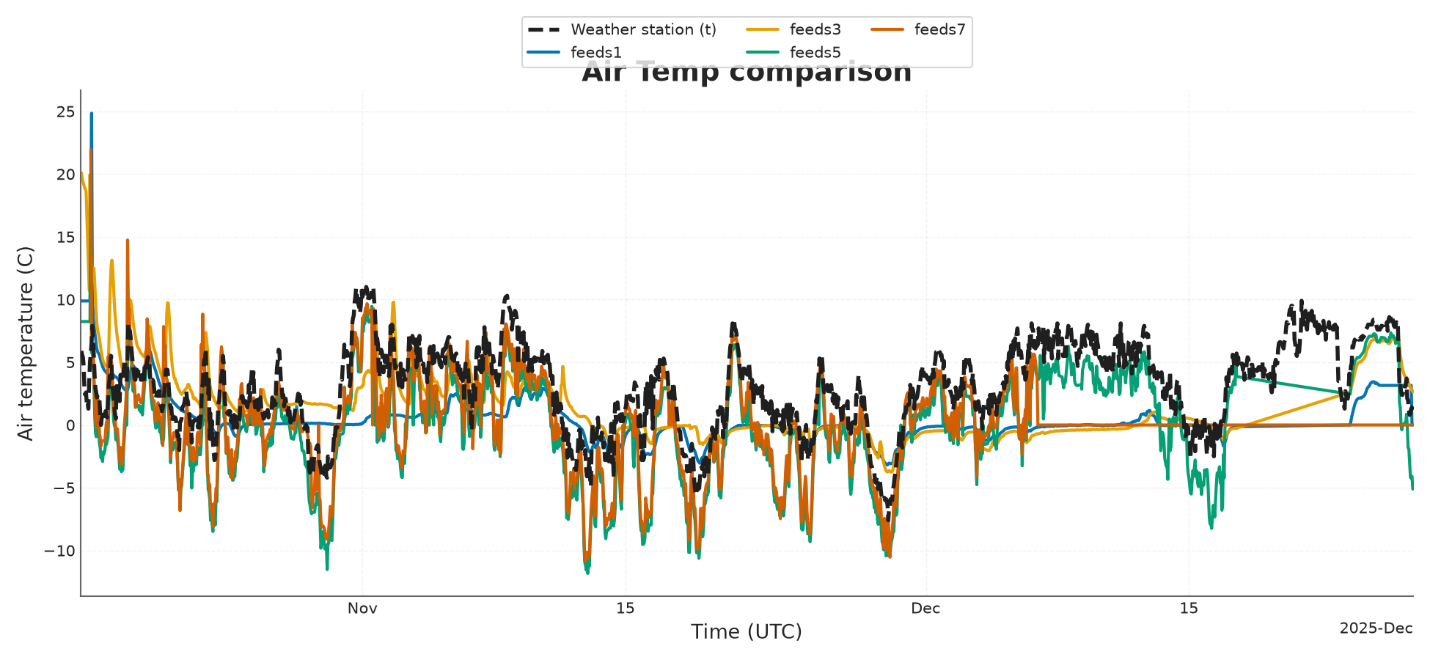
\includegraphics[width=0.48\textwidth,keepaspectratio]{results-image7.png}\hfill
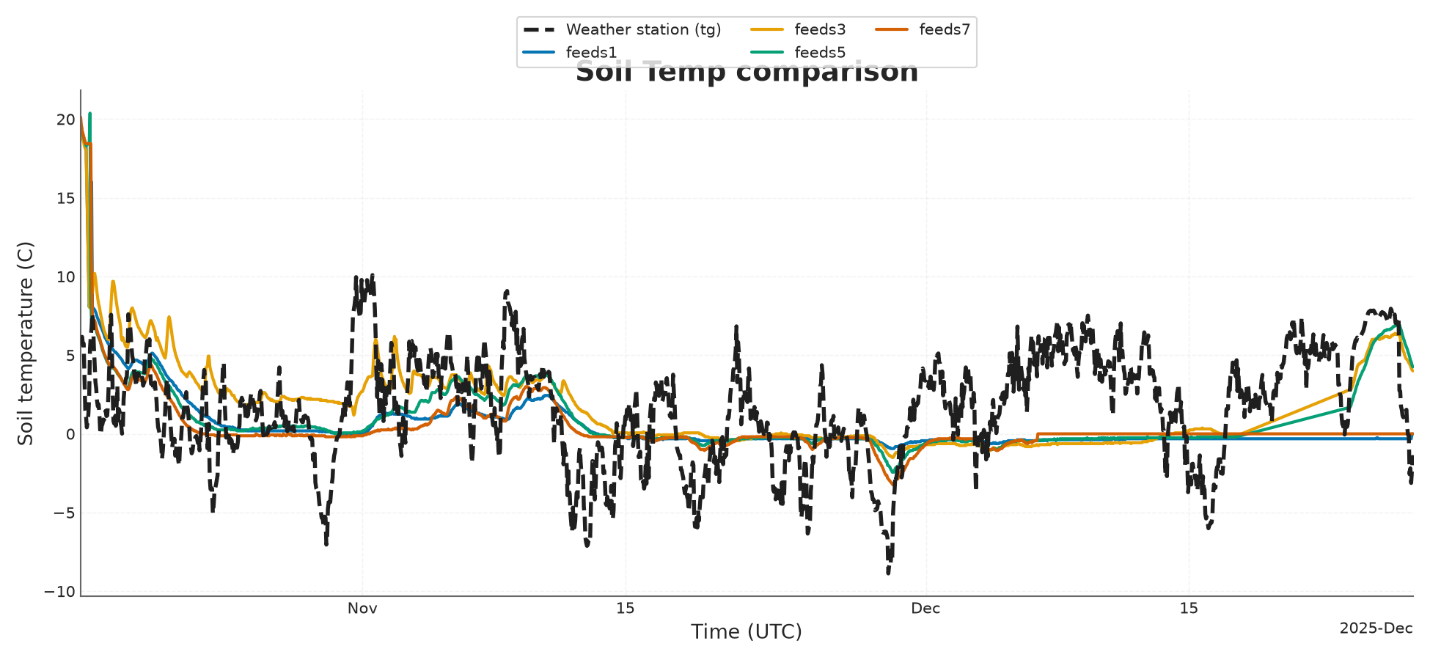
\includegraphics[width=0.48\textwidth,keepaspectratio]{results-image9.png}
\caption{Keldur deployment. Left: air temperature from the four nodes and the S\'amssta\dh ir station (6222). Right: soil temperature from the four nodes and ground-level temperature from the station.}
\label{fig:temps}
\end{figure*}

\subsection{Soil Moisture Calibration}
ADC readings decreased as moisture increased in both tests, as expected for a capacitive sensor. The fitted model is
\begin{equation}
M = 0.0006877\,A^{2} - 0.5961\,A + 127.70,
\end{equation}
where $M$ is gravimetric soil moisture in percent and $A$ is the raw ADC value. Table~\ref{tab:cal} and Fig.~\ref{fig:cal} compare the model with the calibration targets. The in-sample RMSE is 3.01 percentage points. It is a fit error on the data used to derive the model, not an independent validation.

\begin{table}[t]
\caption{Calibration Data (Test 1 Mean of Two Sensors)}
\label{tab:cal}
\centering
\small
\begin{tabular}{@{}cccc@{}}
\toprule
Gravimetric (\%) & Mean ADC & HOBO VWC (m$^3$/m$^3$) & Model (\%) \\
\midrule
0 & 484.89 & 0.01 & 0.35 \\
10 & 319.36 & 0.18 & 7.47 \\
20 & 235.73 & 0.28 & 25.40 \\
30 & 219.97 & 0.335 & 29.85 \\
40 & 197.18 & 0.39 & 36.90 \\
\bottomrule
\end{tabular}
\end{table}

\begin{figure}[t]
\centering
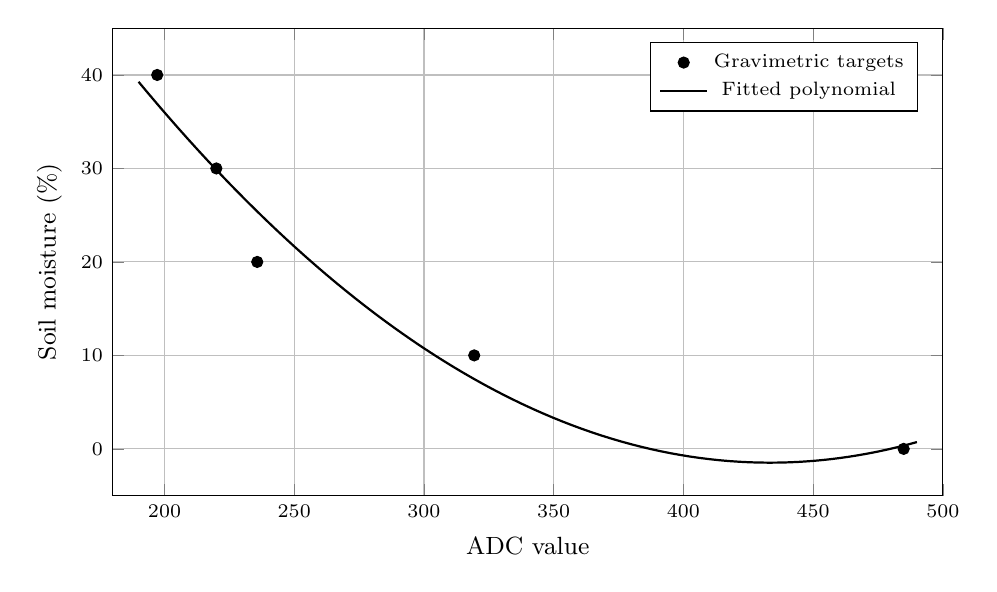
\begin{tikzpicture}
\begin{axis}[
  width=\columnwidth, height=0.62\columnwidth,
  xlabel={ADC value}, ylabel={Soil moisture (\%)},
  xmin=180, xmax=500, ymin=-5, ymax=45,
  grid=major, legend pos=north east,
  legend style={font=\scriptsize}, tick label style={font=\scriptsize},
  label style={font=\small}
]
\addplot[only marks, mark=*] coordinates {(484.89,0) (319.36,10) (235.73,20) (219.97,30) (197.18,40)};
\addplot[domain=190:490, samples=80, thick] {0.0006877*x^2 - 0.5961*x + 127.70};
\legend{Gravimetric targets, Fitted polynomial}
\end{axis}
\end{tikzpicture}
\caption{Second-order calibration of the capacitive sensor over 0--40\% gravimetric moisture.}
\label{fig:cal}
\end{figure}

The HOBO logger reports volumetric water content, whereas the polynomial was fitted to gravimetric moisture. Converting between them requires the soil bulk density, which was not measured, so the HOBO values are used as a reference trend only and no error metric against them is reported.

The calibration soil was a separate Icelandic sample, not soil from Keldur. Most Keldur raw readings lie outside the calibrated ADC range of 197.18 to 484.89; the median raw values were about 527, 575, 768, and 568 for nodes 1, 3, 5, and 7, and only 31.1\% of node 1 and 0.8\% of node 3 readings, and none from nodes 5 and 7, fell within the range. The fitted quadratic has its minimum near $A\approx433$, so values converted outside the range involve extrapolation and are not reliable absolute estimates. They are suitable only as indicative evidence of relative change.

\subsection{Cloud Upload and Local Storage}
Uploads to ThingSpeak consistently returned HTTP 200 OK, with an average upload time of approximately 1--2~s depending on network conditions. These controlled tests do not establish uninterrupted cloud availability during the Keldur deployment. Local SD storage was tested during the earlier campus tests, where logged measurements were used to fill gaps left by missed wireless transmissions. The Keldur SD cards have not been retrieved, so the recovery of missing Keldur records could not be demonstrated.

\section{Discussion and Limitations}\label{sec:discussion}
The results show that a low-cost, concealed LoRa sensor network can collect and deliver soil and environmental data from several turf roofs at a heritage site. Several limits apply to the evidence.

\begin{itemize}
\item \textbf{Lifetime.} The 142-day figure is a nominal calculation from measured state currents and an assumed duty cycle, not a measured lifetime, and it ignores cold-temperature capacity loss.
\item \textbf{Multi-hop performance.} Range tests used single-hop links, and mesh operation was observed only qualitatively. No routes were quantified at Keldur because no packet logs were kept.
\item \textbf{Calibration.} The model is an in-sample fit on a separate soil over 0--40\%, and most field readings fall outside this range. Calibration with site soil and an independent validation set is needed.
\item \textbf{Reference data.} The nearest weather station is 9.75~km from Keldur and lacks soil measurements at depth, so comparisons are contextual.
\item \textbf{Data quality.} Uploaded zero values are placeholders for missing data, some humidity readings were implausible, and the timestamps are ThingSpeak upload times rather than node RTC times.
\item \textbf{Security.} RC4 gives only basic obfuscation and is not a secure encryption mechanism.
\end{itemize}

\section{Conclusion and Future Work}\label{sec:conclusion}
This paper presented a low-power LoRa mesh sensor network with SD-card backup and ThingSpeak integration for monitoring soil conditions under Icelandic turf roofs. The node's calculated average current of 3.08~mA corresponds to an idealized 142-day lifetime on three 3,500~mAh cells. Single-hop LoRa links worked at several locations within about 3~km, the moisture sensor was calibrated over 0--40\% with an in-sample RMSE of 3.01 percentage points, and four nodes delivered valid records from Keldur for approximately 51 to 130 days.

Future work should add base-station logging of packet IDs, RSSI/SNR, forwarding events, and upload status; run controlled multi-hop tests; calibrate with soil from the turf roofs and validate against co-located reference instruments; add remote node-health reporting; test battery performance through winter; improve enclosure and sensor protection; and migrate to a binary packet format with stronger security.

\section*{Acknowledgment}
The author thanks the thesis supervisors, Dr.~Helgi \TH orbergsson and D\'or\'otea H\"oeg Sigur\dh ard\'ottir, and the University of Iceland and the National Museum of Iceland for their assistance and cooperation, and \"Ossur for its support during the studies. This paper is based on the author's M.Sc. thesis at the University of Iceland.

\bibliographystyle{IEEEtran}
\bibliography{references}

\end{document}
